While the overall performance of the LSTM is impressive, it is difficult to make statements about just how impressive without comparing the predictions to other popular forecasting methods. As alluded to in Section \ref{sec:intro}, an Autoregressive Integrated Moving Average (ARIMA) and a Holt-Winters Exponential Smoothing model were fit on the same training data used for the LSTM. The Holt-Winters model used triple exponential additive smoothing and the ARIMA model was fit using the `auto\_arima()' function within the `tsa' package, resulting in a $4^{th}$ order auto-regressive model. Each model was used to forecast 31 days past the training data and were compared to the observed water depths (see Figure \ref{fig:Comparison}).

\begin{figure}[ht]
    \centering
    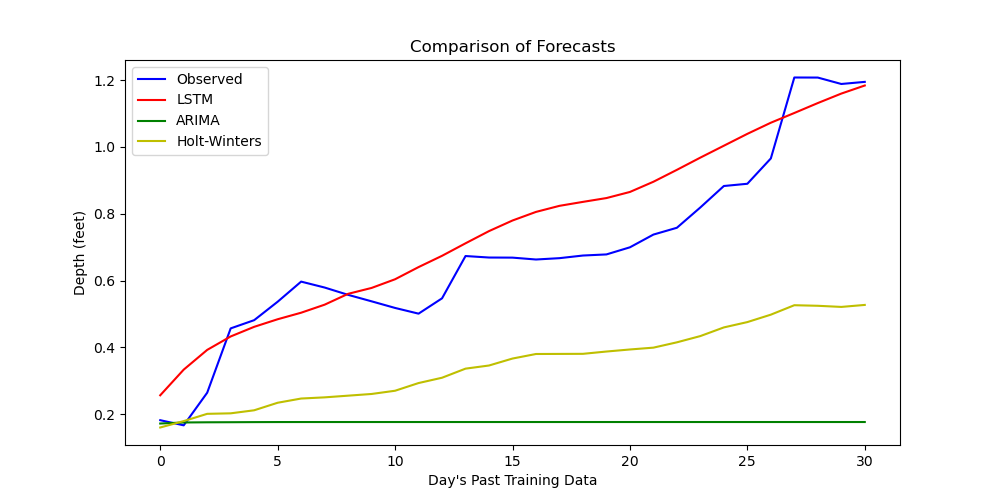
\includegraphics[width=1\linewidth]{"Figures/LSTM_ARIMA_HW.png"}
    \caption{A comparison of 31 day forecasts between the 3 models. Each model was trained on the same data.}
    \label{fig:Comparison}
\end{figure}

While it may seem strange that the ARIMA model predicts a constant trend, this can be explained by the estimated coefficients for the autoregressive components in the model. This constant prediction indicates that the water depth is likely to come back down after a while.